\section{Результаты}

\subsection{Данные выборки}
 
\begin{figure}[H]
	\begin{center}
		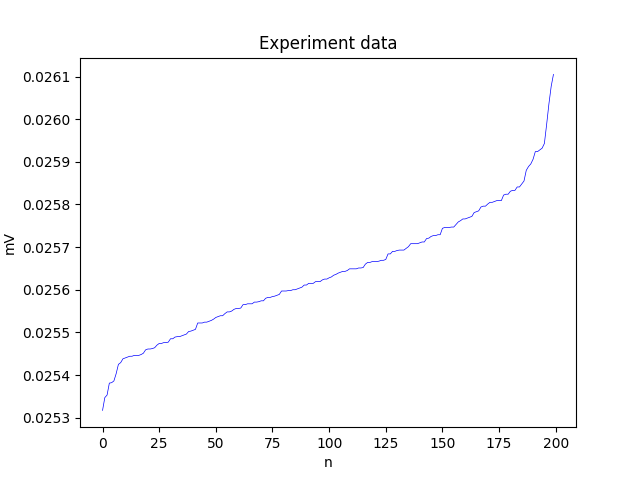
\includegraphics[scale = 0.55]{data.png}
	\end{center}
	\caption{Данные выборки $\bm{X}_1$}
\end{figure}

\begin{figure}[H]
	\begin{center}
		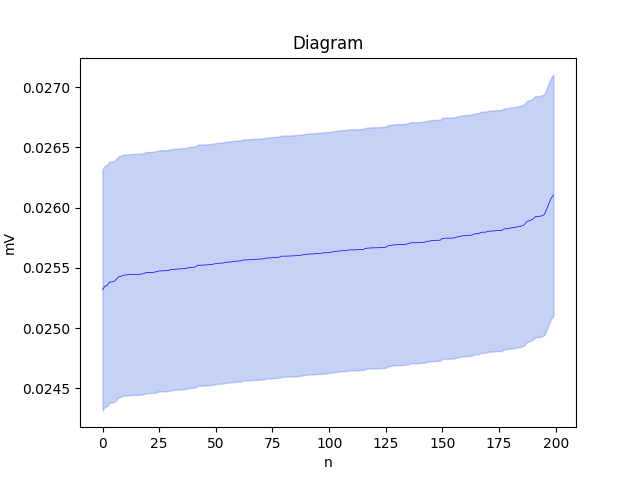
\includegraphics[scale = 0.55]{diagram_beta_None.png}
	\end{center}
	\caption{Диаграмма рассеяния выборки $\bm{X}_1$ с уравновешанным интервалом неопределенности}
\end{figure}

\subsection{Варьирование неопределенности изменений}

При решении задачи линейного программирования были получены следующие результаты: 

\begin{equation*}
	\beta_0 = 0.025, \beta_1 = 3.439 \cdot 10 ^ {-6} 
\end{equation*}

\begin{equation*}
	w_1 = (w^{1}_1, \ldots, w^{n}_1), \sum\limits_{i=1}^{n} w^{i}_1 = 200.169
\end{equation*}

\begin{figure}[H]
	\begin{center}
		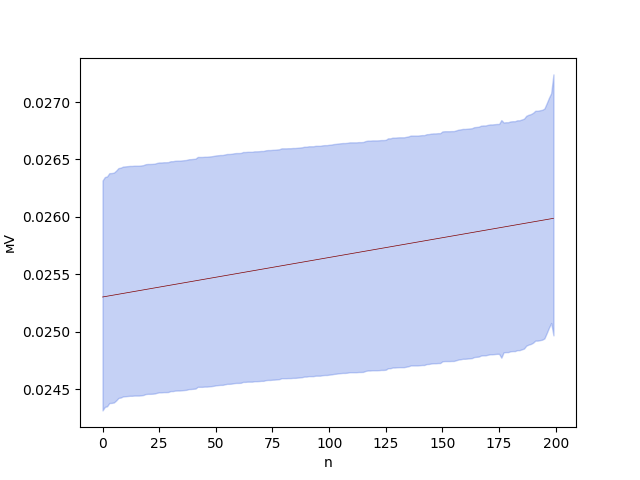
\includegraphics[scale = 0.55]{diagram_and_regress_1.png}
	\end{center}
	\caption{Диаграмма рассеяния выборки $\bm{X}_1$ и регрессионная прямая по модели}
\end{figure}

Красным цветом обозначена регрессионная прямая модели. 

\subsection{Варьирование неопределенности изменений с расширением и сужением интервалов}

При решении задачи линейного программирования были получены следующие результаты: 

\begin{equation*}
	\beta_0 = 0.025, \beta_1 = 2.200 \cdot 10 ^ {-6} 
\end{equation*}

\begin{equation*}
	w_0 = (w^{1}_0, \ldots, w^{n}_0), \sum\limits_{i=1}^{n} w^{i}_0 = 32.546
\end{equation*}

\begin{figure}[H]
	\begin{center}
		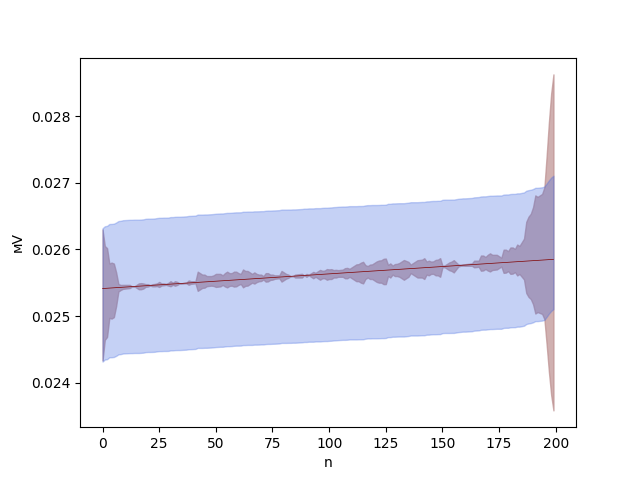
\includegraphics[scale = 0.55]{diagram_and_regress_0.png}
	\end{center}
	\caption{Диаграмма рассеяния выборки $\bm{X}_1$ и регрессионная прямая по модели}
\end{figure}

Розовым цветом обозначены скорректированные интервалы выборки $\bm{X}_1$, голубым - первоначальные интервалы, красным цветом обозначена регрессионная прямая. 

\begin{figure}[H]
	\begin{center}
		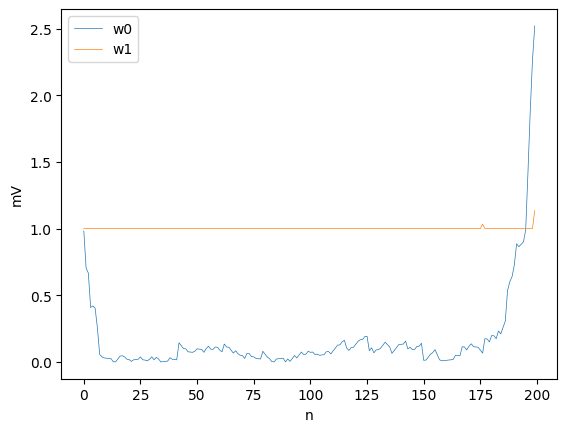
\includegraphics[scale = 0.55]{w0_w1.png}
	\end{center}
	\caption{Векторы $w_0$ и $w_1$}
\end{figure}

\subsection{Анализ регрессионных остатков}

\begin{figure}[H]
	\begin{center}
		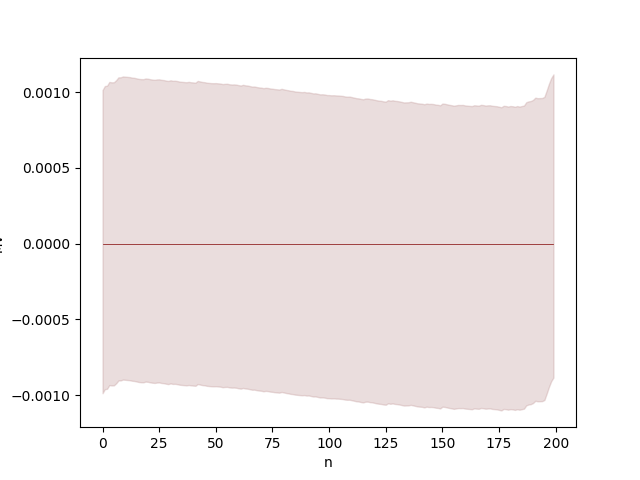
\includegraphics[scale = 0.55]{analysis_of_regression_residuals_1.png}
	\end{center}
	\caption{Диаграмма рассеяния регрессионных остатков для модели без сужения интервалов}
\end{figure}

\begin{figure}[H]
	\begin{center}
		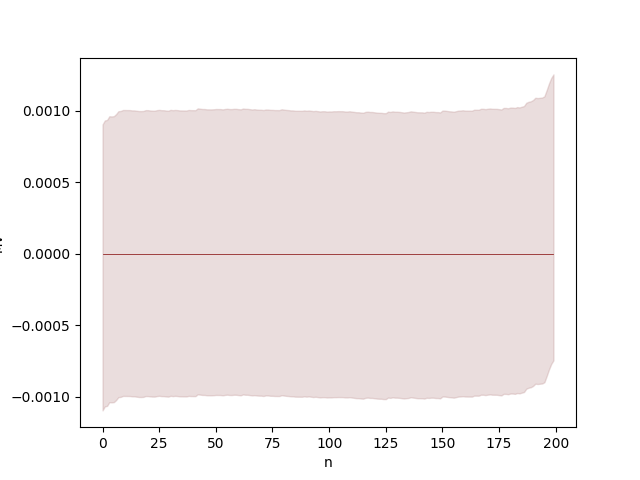
\includegraphics[scale = 0.55]{analysis_of_regression_residuals_0.png}
	\end{center}
	\caption{Диаграмма рассеяния регрессионных остатков для модели с сужением и расширением интервалов}
\end{figure}

\begin{figure}[H]
	\begin{center}
		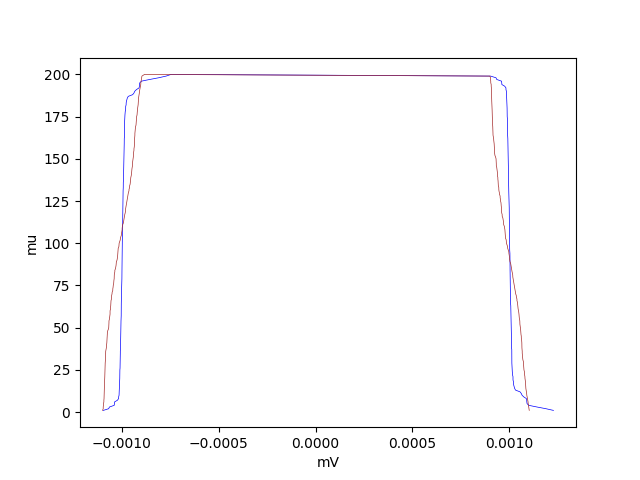
\includegraphics[scale = 0.55]{mu.png}
	\end{center}
	\caption{Частоты элементарных подинтервалов регрессионных остатков при вычислении моды для двух моделей}
\end{figure}

\textbf{Красный график} -- график частот элементарных подинтервалов регрессионных остатков при вычислении моды модели без сужения интервалов. \\
\textbf{Синий график} -- график частот элементарных подинтервалов регрессионных остатков при вычислении моды модели с сужением и расширением интервалов. \\

Меры совместности регрессионных остатков: \\

\begin{tabular}{c c}
	mode $\bm{X}^0 = [-0.0007, 0.0009]$ & $\bm{J}_i(\bm{X}^0) = 0.7020$ \\
	mode $\bm{X}^1 = [-0.0008, 0.0009]$ & $\bm{J}_i(\bm{X}^1) = 0.8043$ \\
\end{tabular}

Здесь $\bm{X}^{0,1}$ -- регрессионные остатки выборки $\bm{X}_1$, вычисленные с использованием разных условий оптимизации. \\

\subsection{Информационное множество задачи} 

\begin{figure}[H]
	\begin{center}
		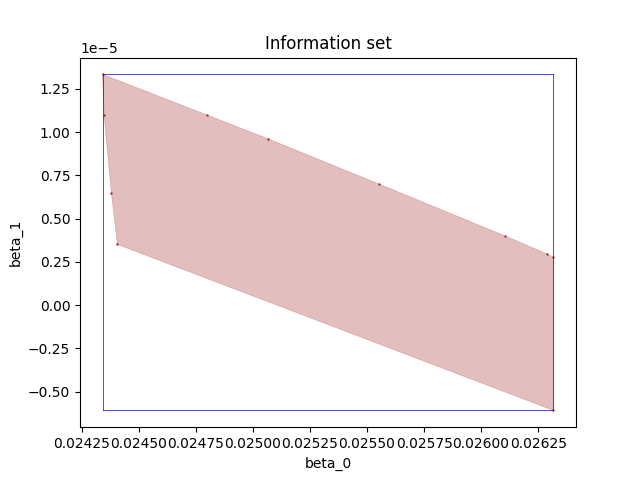
\includegraphics[scale = 0.55]{inform_set.png}
	\end{center}
	\caption{Информационное мноежство задачи по заданной модели -- красный брус, интервальная оболочка -- синий брус}
\end{figure}

\subsection{Коридор совместных зависимостей}

Внешние интервальные оценки параметров модели: 

\begin{equation*}
	\text{mid} \beta_0 = [2.4341e-02,2.6317e-02]
\end{equation*}

\begin{equation*}
	\text{mid} \beta_1 = [-6.0905e-06,1.3344e-05]
\end{equation*}

Подставляя эти значения в уравнение регрессии, получаем:

\begin{equation}
	\bm{x}(k) = \text{mid} \beta_0 + \text{mid} \beta_1 \cdot k
\end{equation}

\begin{figure}[H]
	\begin{center}
		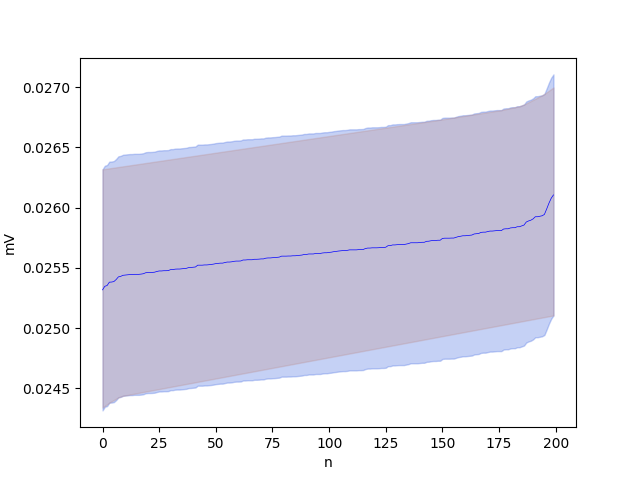
\includegraphics[scale = 0.55]{corridor_of_joint_dependencies.png}
	\end{center}
	\caption{Коридор совместных зависимостей}
\end{figure}

\subsection{Прогноз вне области данных}

\begin{figure}[H]
	\begin{center}
		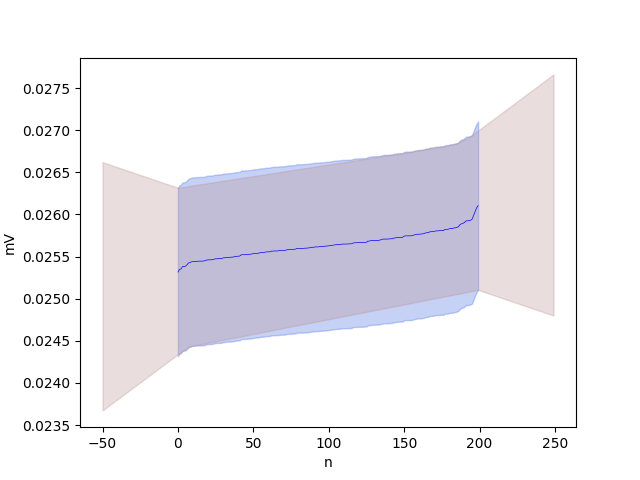
\includegraphics[scale = 0.55]{corridor_of_joint_dependencies_prediction.png}
	\end{center}
	\caption{Коридор совместных зависимостей. Построение прогноза}
\end{figure}


